\section{Applications}
\label{sec:apps}
% In this section we discuss three applications we wrote that use the infrastructure we set up inside a building on campus.
% The building is a 7-story, 141,000 square-foot building.  We tagged 351 items spread over 139 rooms throughout all floors.
% There are WiFi access point spread throughout the entire building, providing ubiquitous access to a network throughout.
% Cellular coverage is also available throughout most of the building as a secondary option for connecting to a network.

In this section we discuss three applications deployed on top of our infrastructure.
The first is an energy auditing application.  The goal of the application is to quickly collect,
organize, and understand plug-loads, also known as miscellaneous
electrical loads (MELs), in the building.
The application provides scalability of the inventory collection process where there previously was none.
Various governmental agencies have conducted field studies of this
sort in order to characterize these loads, but they are severely
limited by the effort involved in obtaining the
inventory\cite{***http://www.efficientproducts.org/reports/plugload/Revised_Office%20Plug%20Load%20Report_PIER_500-06-007_RevApril2011.pdf
                                stevel}. 
 And, the inventory quickly becomes stale as items are moved and
 changed, further frustrating longitudinal studies.  Our goal is not
 just to facilitate the field studies but to make the audit a natural
 offshoot of using the appliances such that it can be used as part of
 an organization energy management strategy without expertise in
 energy auditing.
A second-order result of the audit in the infrastructure it leaves deployed.  We used the deployment
to implement two more applications.  The energy item scanner application gives historical energy information
for any item that the user swipes.  Items include physical objects \emph{and} spaces. Since spaces do not directly 
consume energy, they embody notion of an aggregate.
Similarly, personal energy metering embodies the notion of an aggregate or a family of aggregates.  That is
our the third application we present.

For each we discuss the fundamental challenges with respect to mobility, consistency management, or aggregation and how
our use of gestures and interference were used to address these issues.  We also discuss how the underlying entity-relationship
graph is used to deal with a dynamic set of constituents when computing aggregates.

% We collected both power rating information as well
% as live metering information.  The second application, the energy-view item scanner, builds off the first, allowing users
% to swipe the QR code of an item and view the power-trace and power-rating recorded for that item.  It is also
% used to view aggregates across space; you can scan a floor and see the aggregate data for that floor over time.  
% The third is a personal energy accountant.  This application allows users to virtually tag items that belong to them 
% and view their personal energy consumption, aggregated across all the devices they own.

\subsection{Energy Audit}
\label{sec:eaudit}
Nationally, MELs consume about third of the energy in building in the United States~\cite{eia:2010}.  However,
given the nature of these electrical loads, collecting enough information quickly from hundreds of disparate
loads spread throughout the building simply does not scale.  In~\cite{lbnlmels}, they describe the major challenge
in collecting device inventory for studying MELs and state the the process simply does not scale to large buildings.

The energy audit application addresses this issue.  We leverage the occupants, particularly the ones with mobile phones
to scale the inventory collection processes.  Once they download our application and print a QR code from our site, they
attach it to an item and register it using the phone.  This scales to any building size, as long as the number of occupants
scales with the number of devices and the size of the building.

Execution of the audit builds the entity-relationship graph.  Each time a new item or space is registered a node is added
to the graph.  The first objects we need to learn about are spaces and how they are inter-related.  StreamFS
was pre-populated with a directory to record that information.  A user can add a new room if either the room has no tag
or the current tag is not registered (which they can determine by swiping it).  Once a room is added, objects within that
room can be added.  Figure~\ref{fig:msfsv2} shows a screen shot of the auditing application.  
We also applied a classification hierarchy on the objects using a MELs taxonomy~\cite{taxonomy}
incorporated into StreamFS as a directory.

Note, however, that in order to add an object, we need to know where you are.  That is the main piece of contextual information
that must be deduced or reported.  Prior work has used indoor WiFi~\cite{radar}, learning-based approach~\cite{wigem}, 
and alternative infrastructure~\cite{cricket}.  However, we took a simpler approach:

\begin{enumerate}
\item The person swipes into a space, setting it as their conext for adding new objects or
\item They swipe an, whose location we already know, and we use that to infer their current location.
\end{enumerate}

This approach is much simpler than prior work, but just as effective.  
% It also involves the user in the check-in process rather
% than the infrasture learning about the user.
% It also empowers the person to get involved
% in processes, forcing them to think about the energy problem through explicit participation in the use of the application.


%Restering an object or space adds a node to the entity-relationship graph that represents the physical state of the world.  
%Because each of the physical object are spread throughout the building, 
%maintaining consistency is fundamentally hard and unscalable without occupant participation.  
%In addition, in constructing the relationship graph, the main piece of information is where the object is in the building.  

% To start we need to capture the objects and relationship between them.  Specifically, we set up the hierarchical organization of
% objects with the building at the root, followed by \emph{spaces} and \emph{inventory} within the building, and data streams at the leaves.
% The spaces subtree is the hierarchical organization of floors, rooms, and areas on those floors.  The inventory is a folder where
% each of the physical objects is placed.  We used symbolic links to associate items in the inventory with the location
% they are in.  In addition, we added a categorical subtree to ease aggregation with respect to the category of devices.
% For personalized accounting, users created their own folder that points to items that belong to them.
% Figure~\ref{fig:hierarchy} shows a partial view of the hierarchy that supports our applications.

% After the hierarchy is constructed, we place QR codes on objects in the world and register them.  The registration process
% for locations includes the following steps:

% \begin{enumerate}
% \item Place QR code somewhere in the space.
% \item Scan QR code.
% \item Choose which space it represents.
% \end{enumerate}

% \vspace{0.04in}

% The basic set of spaces that initially inputted by hand are the building and the floors.  We placed QR code on the entrance of the building
% and the main door to enter the floor.  Once each of these spaces is registered, the user can set their context by swipe the QR code tag.
% When rooms are added, the user first scans the tag for the floor they are on, then they place a tag on the room and they enter information
% about the room.  For items, the process is the same.  We scan the room we are in, place the tag on the object and enter information about
% object.

% The initial location scan sets the context.  For example, when you first enter a building, you scan the QR code associated with that building.
% The {\tt URL} fetched from the QR code is first resolved.  

\subsection{Inter-relationship capture}
\label{sec:binding}
%Talking about how you bind an item and meter.
There is a special relationship between meters and items.  Items are attached to meters, but more importantly, the data
collected from the sensor \emph{represents} the underlying dynamics of some physical measurement related to the item.  A power 
meter attached to a television gives us the power profile of that television over some time period.  Furthermore, if the meter 
is removed
from the television and attached to another item, that change needs to be recorded, so that we do not attribute the power
trace from the second item to the television.  There are also items are that attached to each other that can affect how we 
aggregate feeds.  For example, in our deployment, we sometimes connect meters to power-strips, which have multiple items
attached to them.  The meter serves as a proxy-aggregate for the attached the power strip that's attached the meter.

%FILL IN WITH REAL GRAPH
\begin{figure}[htb!]
\begin{center}
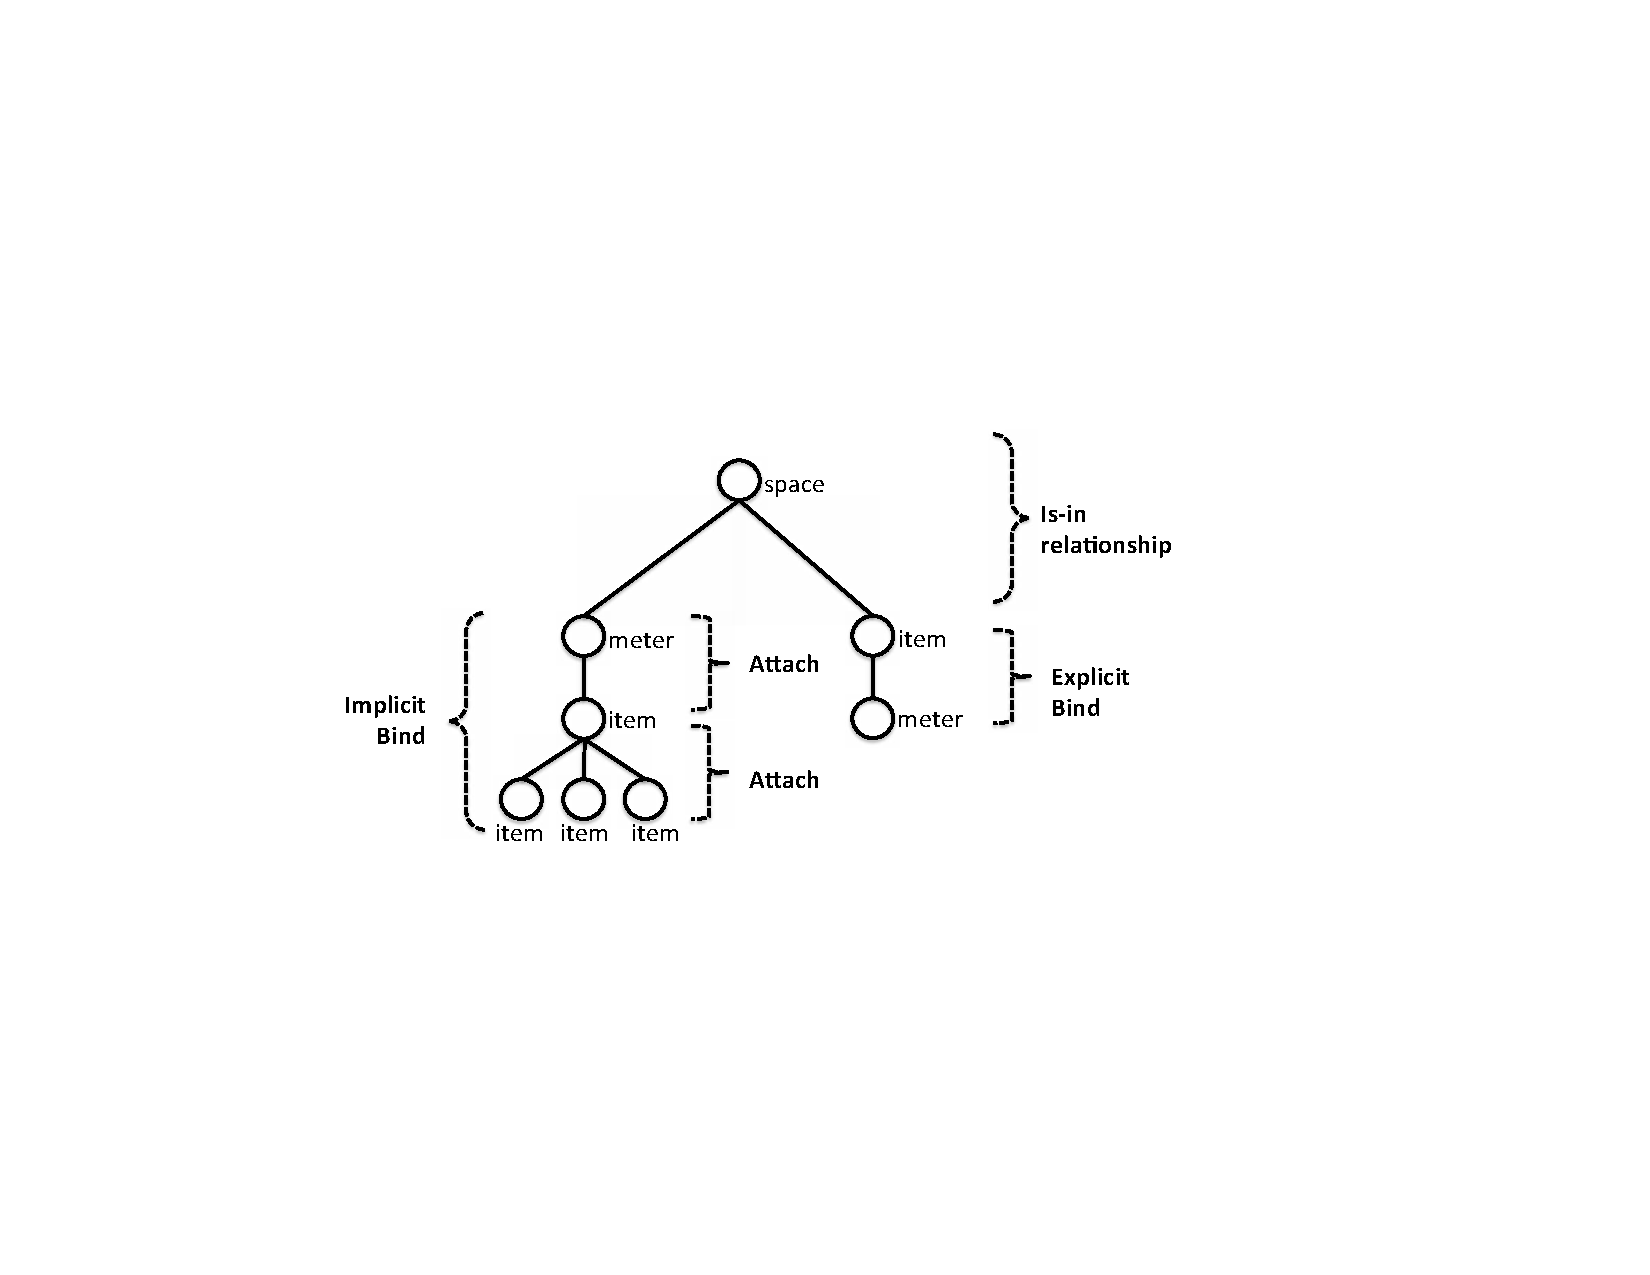
\includegraphics[scale=0.55]{figs/bindattachstructs}
\caption{This diagram shows the relationship capture between the objects and locations in the building for the 
energy audit application.  Children of a space node have an ``is-in'' relationship with the space.  An item
with another item as a child have a ``attached'' relationship and meters attached to items are bound to each other.
Note, this is a \emph{subset} of the relationship diagrams generated across our three applications.}
\label{fig:attachandbind}
\end{center}
\end{figure}

Both types of relationship are interpretted by how nodes are symbolically linked.  If a meter is the child
of an item, it is bound to that item and can be used as a proxy for measurements pertaining to that item.
If an item is a child of a meter, it is attached to the meter, but the measure is not taking measurements
pertaining to the item, instead if it taking measurement of the children of the item.  Figure~\ref{fig:attachandbind}
highlights the two kinds of relationships interpretted by our applications.  The one of the left shows
a bind relationship while the one of the right shows and attach relationship.
To bind or attach the gesture is the same.  You first swipe the item the swipe the meter and press a button to either
un/attach or un/bind.

% \subsection{Energy Auditing}
% The energy auditing application was written to capture all of the plug-load devices in a building.  Included it their
% capture is information about the plated power-draw of the device, if available, its make, model, and category.
% The capture consists of walking around the building with a set of QR codes, registering each of the rooms and items
% within them.  For each room you enter the name of the room.  The floor is indicated explicitly through a swipe of the buidling
% floor tag.  Once inside the room each electrical device is tagged and registered.  To register the item the QR code needs
% to be added, followed by a small form that is filled out by the auditor.  The form includes information for the name
% of the device and the power rating or current draw.  

Figure~\ref{fig:msfsv2} shows two screenshot of the auditing interface.  The first page is a list of options and the second is
the registration page.  Once the page is filled out, the user scans the QR code once again and the item is added to the inventory.
In addition, the QR code tag identifier is added to the `qrc' directory and symbolically linked to the newly added item
in the inventory directory.  Finally, a symbolic link is create in the directory for the room that also points to the item
just added to the inventory.

\begin{figure}[htb!]
\begin{center}
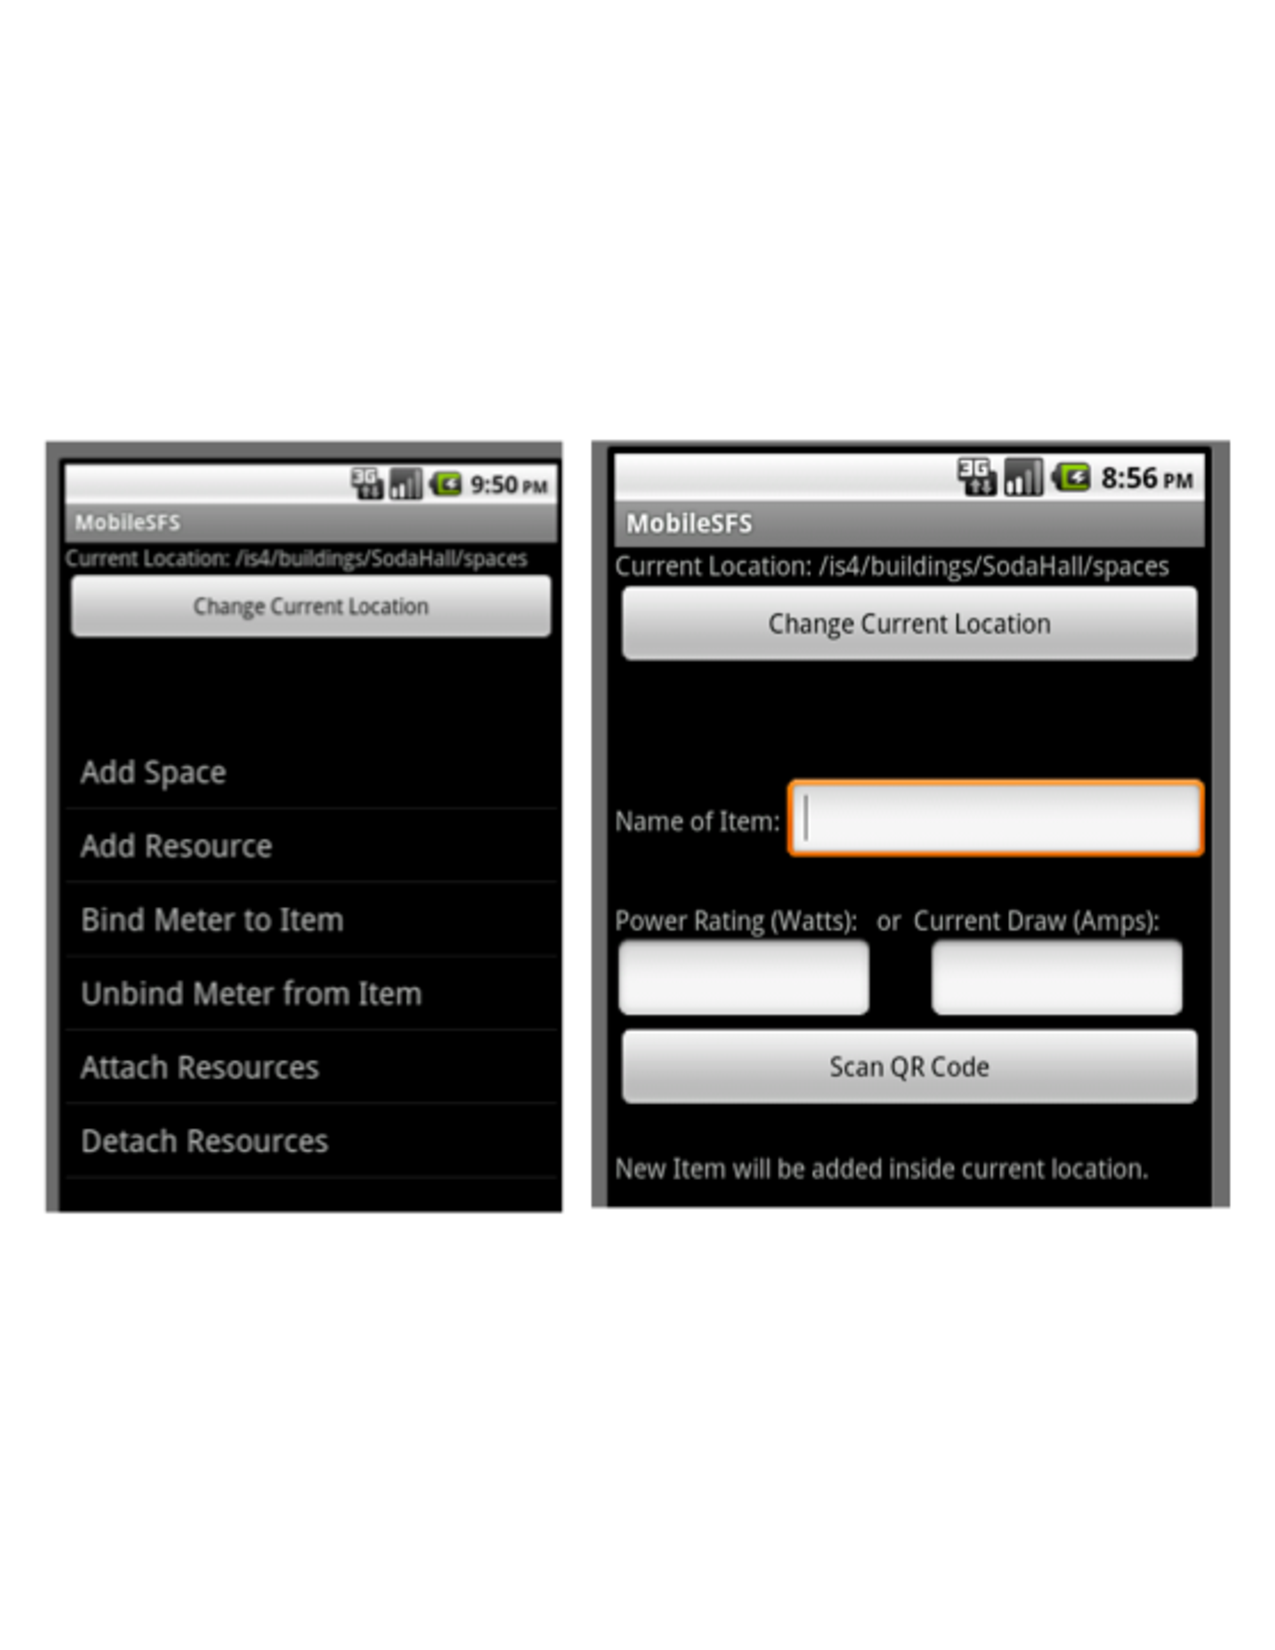
\includegraphics[scale=0.39]{figs/msfsv2screens}
\caption{}
\label{fig:msfsv2}
\end{center}
\end{figure}

Auto-classification was done using the same of the item as well.  In addition to the spaces, qrc, and inventory directories
there is also a taxonomony directory.  Items with a given prefix were classified as being items in a particular
directory of the taxonomy.  A symbolic link was also created from the corresponding node in the taxonomy, that most closely
matches the item, to the item node.

In our current deployment we use the link gesture to link an appliance
to the wireless power meter that monitors its consumption.  In the
future, such capability might well be built into the appliance
itself.  However, other contextual information about the appliance and
its relationship to the space and the people that use the space is
likely to remain.

\subsubsection{Results}
This application was focused on capturing the physical, energy-consuming objects, describing them in various way
and coupling that information with live streaming power data.  Figure~\ref{fig:devicecount} shows the breakdown of the
types of devices that were recorded by the energy auditing application.  Since this data was collected from a office
building, most of the device were actually LCD screens.

\begin{figure}[htb!]
\begin{center}
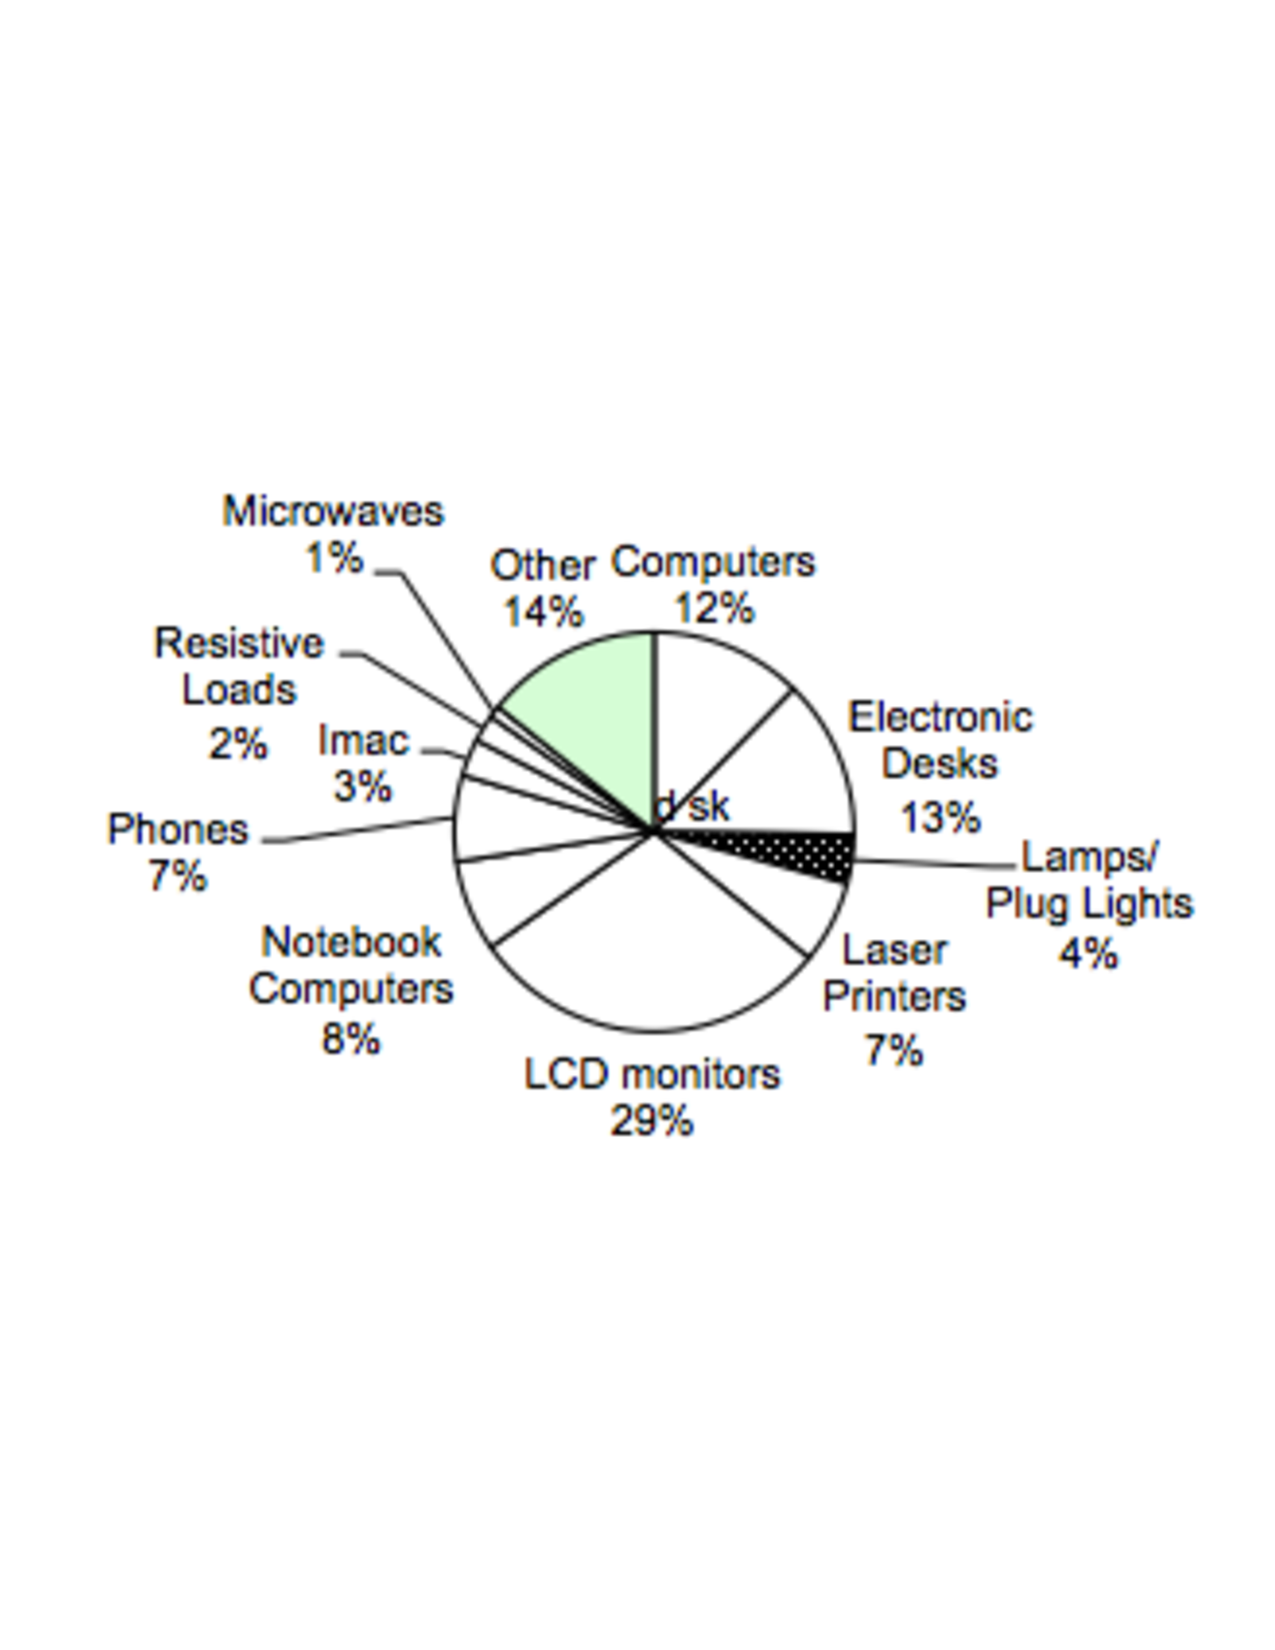
\includegraphics[scale=0.42]{figs/devicecount}
\caption{The percentage breakdown of the devices that were captured.}
\label{fig:devicecount}
\end{center}
\end{figure}

Although most of the items are static, a good number of them are moved by their owners pretty often.  For example, 8\%
of the device were classified as notebooks.  When the owner leaves the room or building, they usually take their notebook
with them.  This kind of information should be recorded using the auditing application.  By simply swiping QR code for the notebook
and clicking the `leave' button, the item is kept in the inventory for the building, but the symbolic link from the 
room to the item is deleted.

\begin{figure}[htb!]
\begin{center}
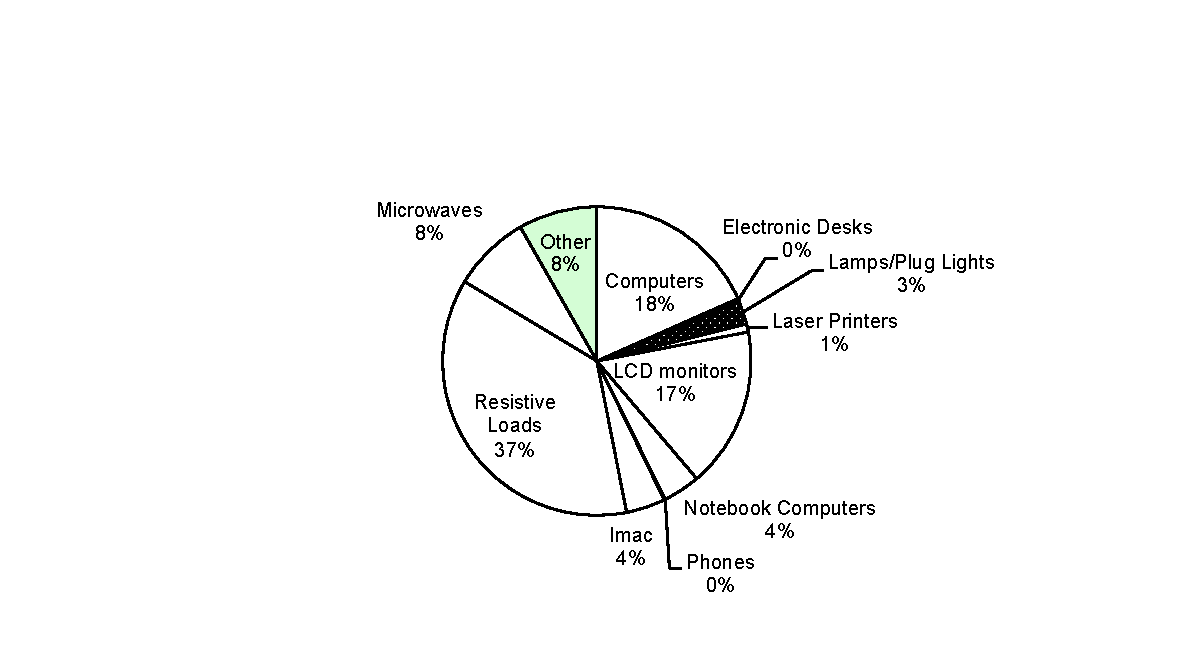
\includegraphics[scale=0.7]{figs/PIE_CHART_SANS_WATTS}
\caption{Device power draw in Watts.}
\label{fig:piechart}
\end{center}
\end{figure}

Figure~\ref{fig:piechart} shows the power-draw distribution.  Interestingly, although the category of devices that 
fall under `resistive loads', which includes things like space heaters
and toaster ovens, make up only 2\% of the items recorded, they
account for a much larger fraction of the total power-draw.
% Axed the bogus stuff about multiplying something by nameplate.  It
% all depends on usage cycle anyways.  At best hope this gets in and
% this cruddy stuff gets fixed.  Currently it is totally bogus


\begin{figure}[htb!]
\begin{center}
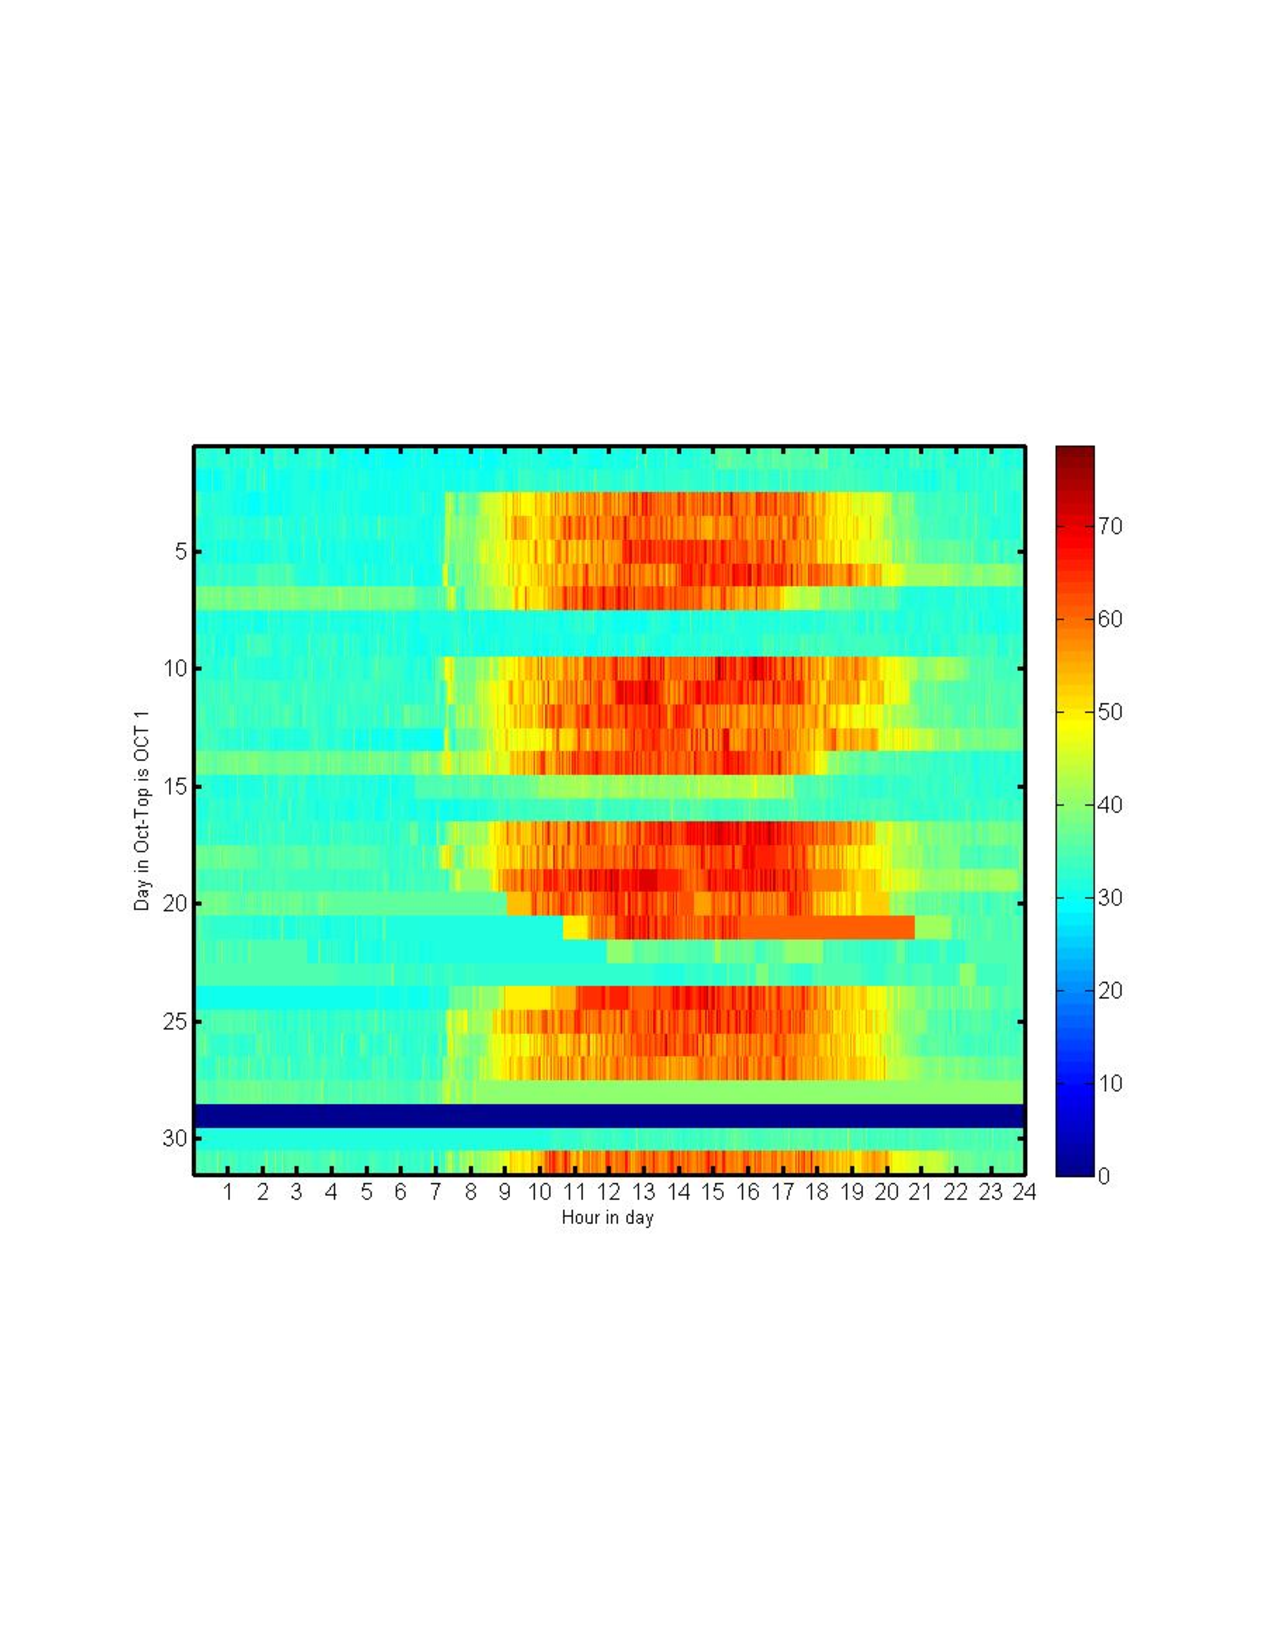
\includegraphics[scale=0.49]{figs/Aggregate_SDH_OCT_PLUG_LOADS}
\caption{Power heatmap generated from the data obtained from meters attached to plug-load devices throughout the building.  
Red zones are locations where the highest amount of power is being consumed.}
\label{fig:plugloadheatmap}
\end{center}
\end{figure}

Figure~\ref{fig:plugloadheatmap} was generated using actual live, plugload data throughout the day during the entire month
of October.  The x-axis shows the hour of the day, while the y-axis indicates the day in october.  This data was aggregated
over hourly period by summing all the plug-load data collected over that hour.  Notice the busiest times between 10am and 
about 6pm.  There's also a clear view of the weekends.

% \begin{figure*}[htb!]
% \begin{center}
% 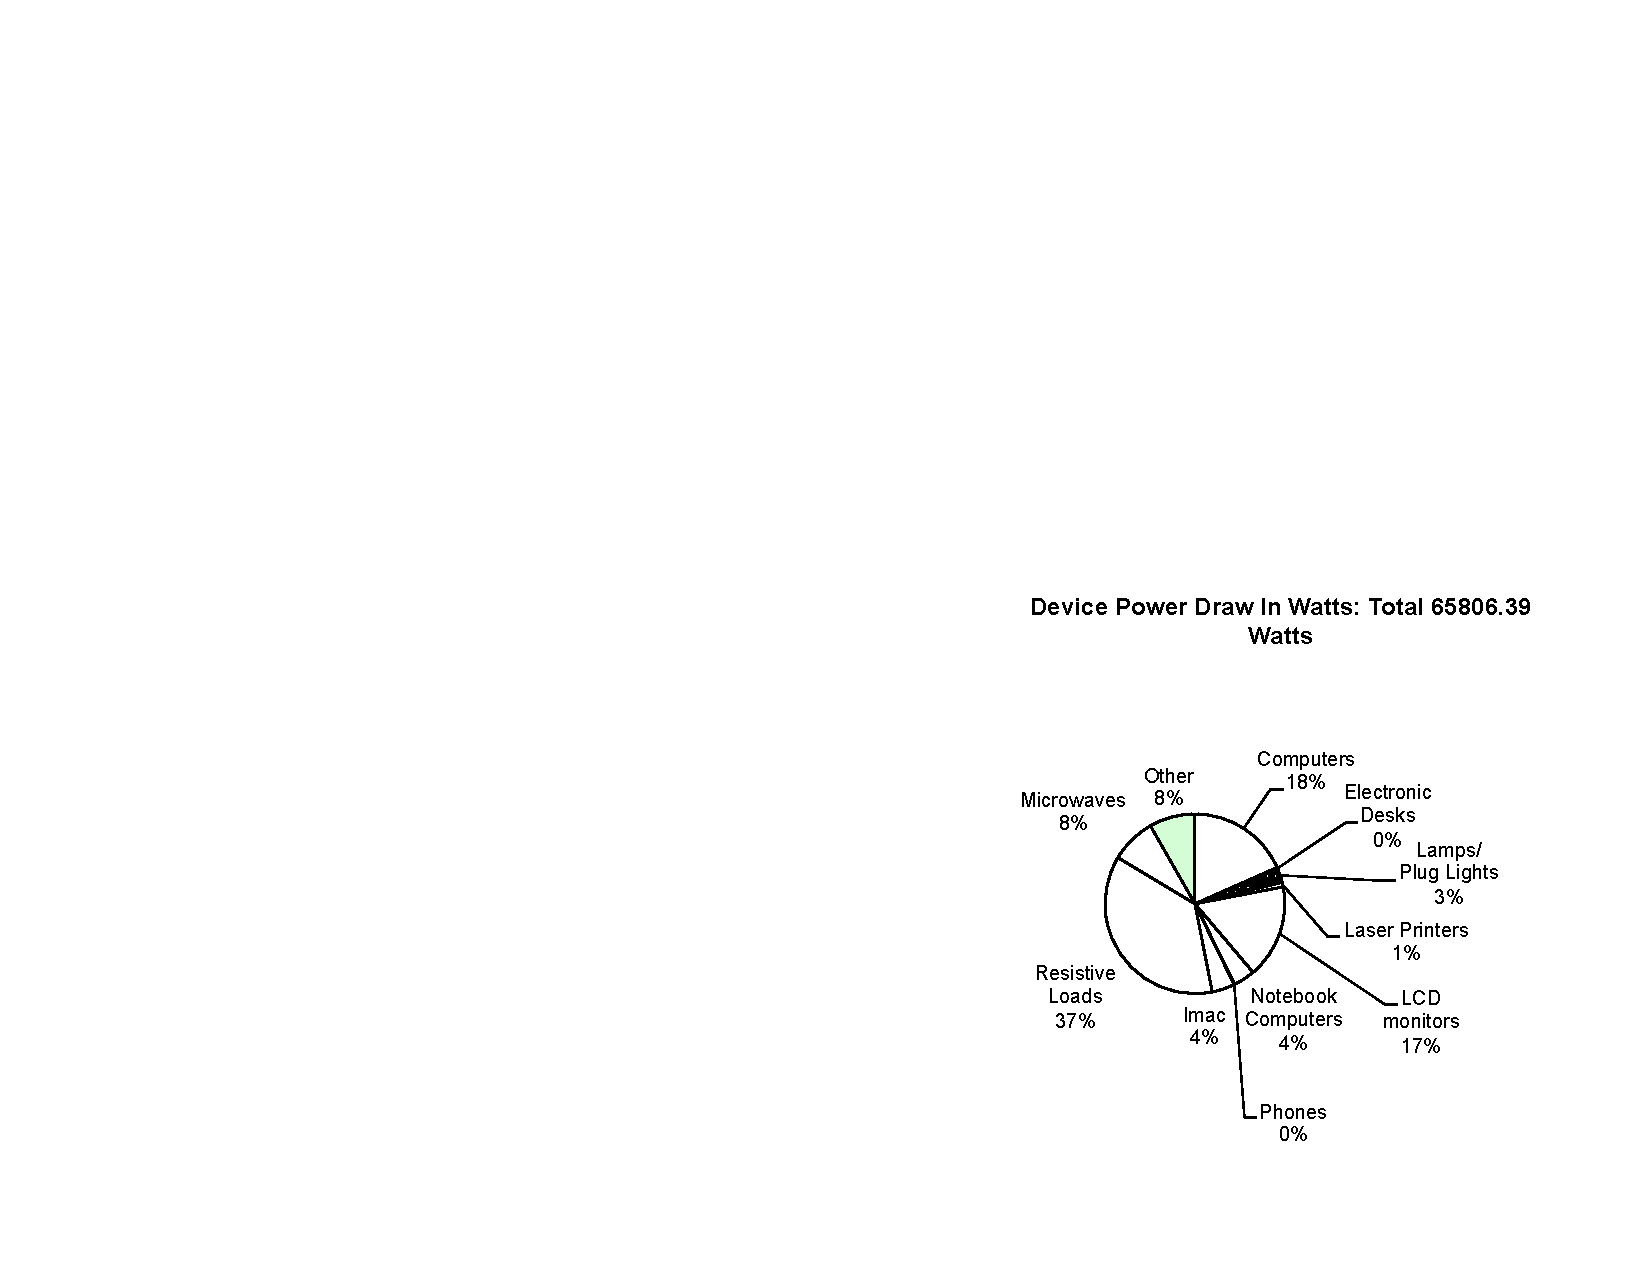
\includegraphics[scale=0.8]{figs/device_info02}
% \caption{}
% \label{channelcomp}
% \end{center}
% \end{figure*}

\begin{figure}[htb!]
\begin{center}
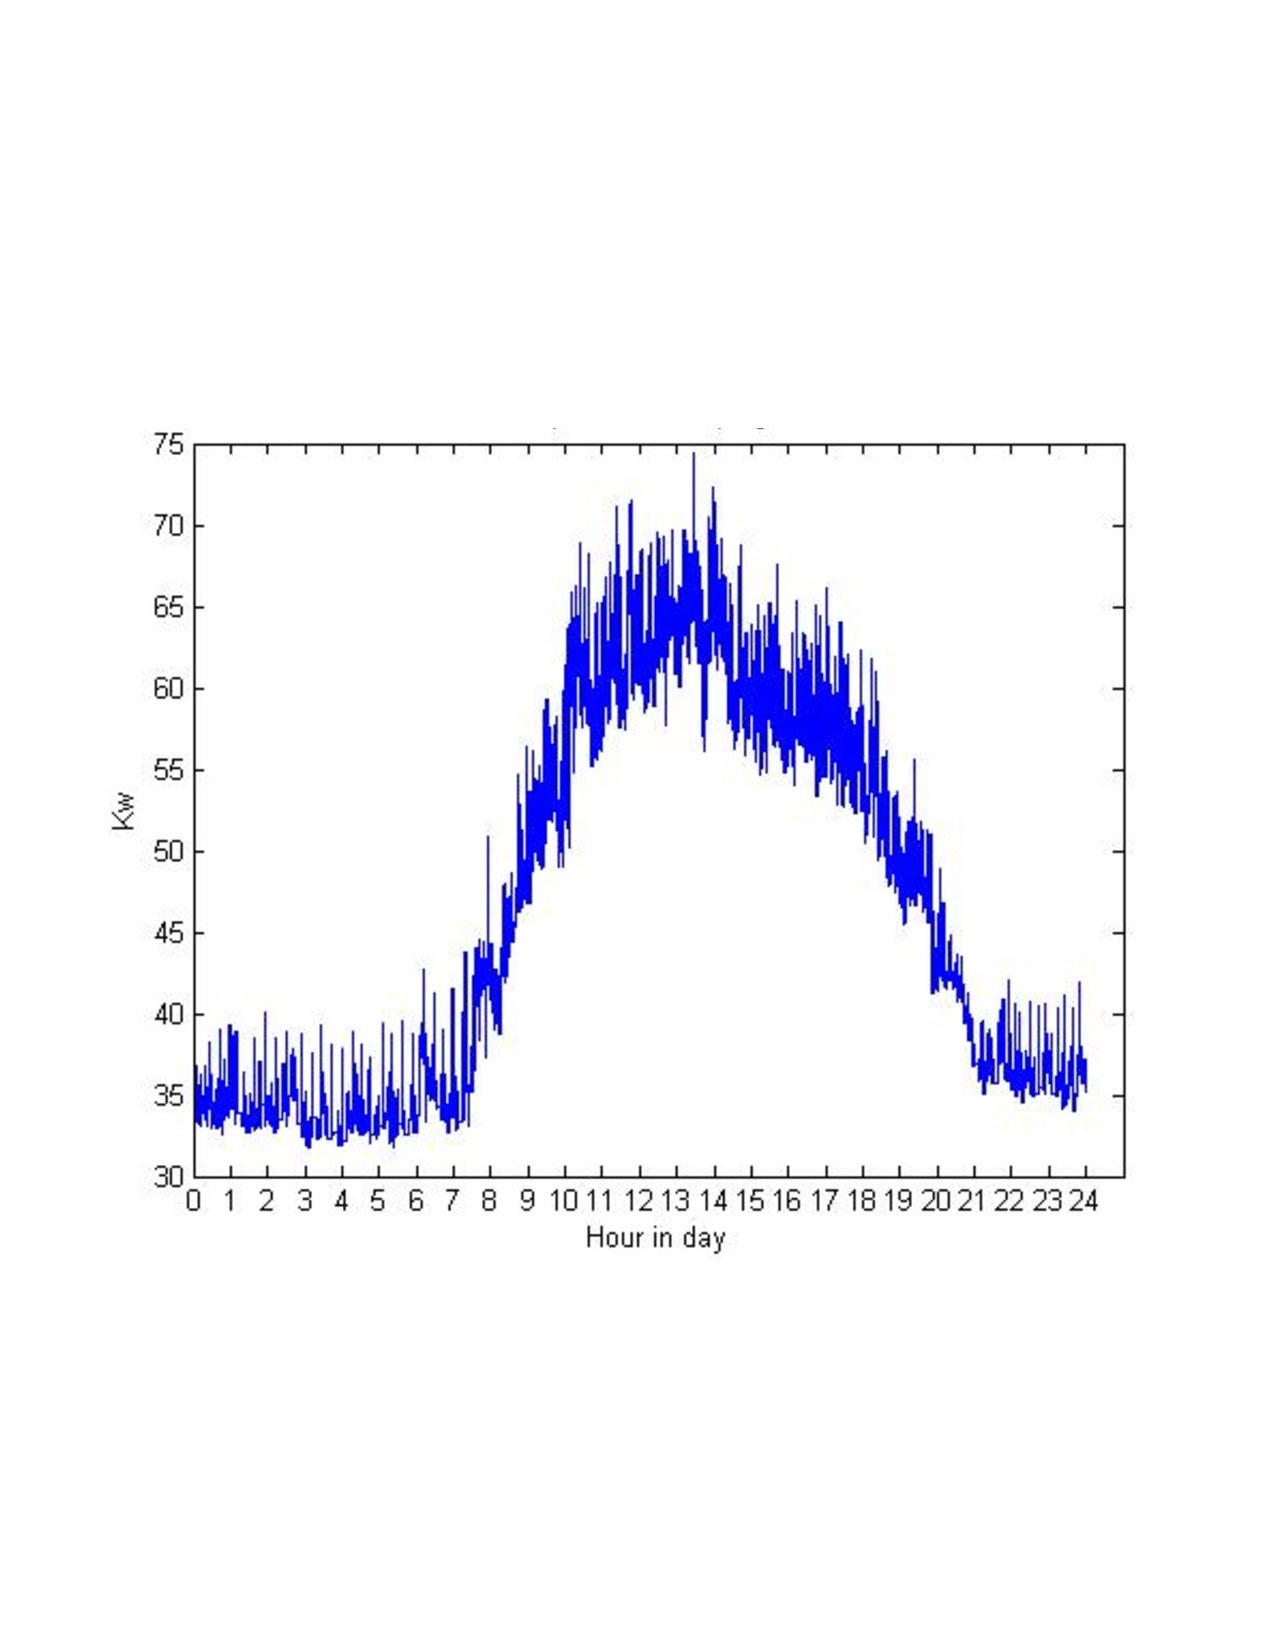
\includegraphics[scale=0.4]{figs/WholeOct12}
\caption{Whole building power draw on October 12th.}
\label{fig:wholebuilding}
\end{center}
\end{figure}

Figure~\ref{fig:wholebuilding} shows the whole building power-draw feed.  This meter was obtained through the building
management system and added to the audit.  Notice how the peak and low times correspond to the patterns observed
in the monthly plug-load heat map.

% \begin{figure}[htb!]
% \begin{center}
% 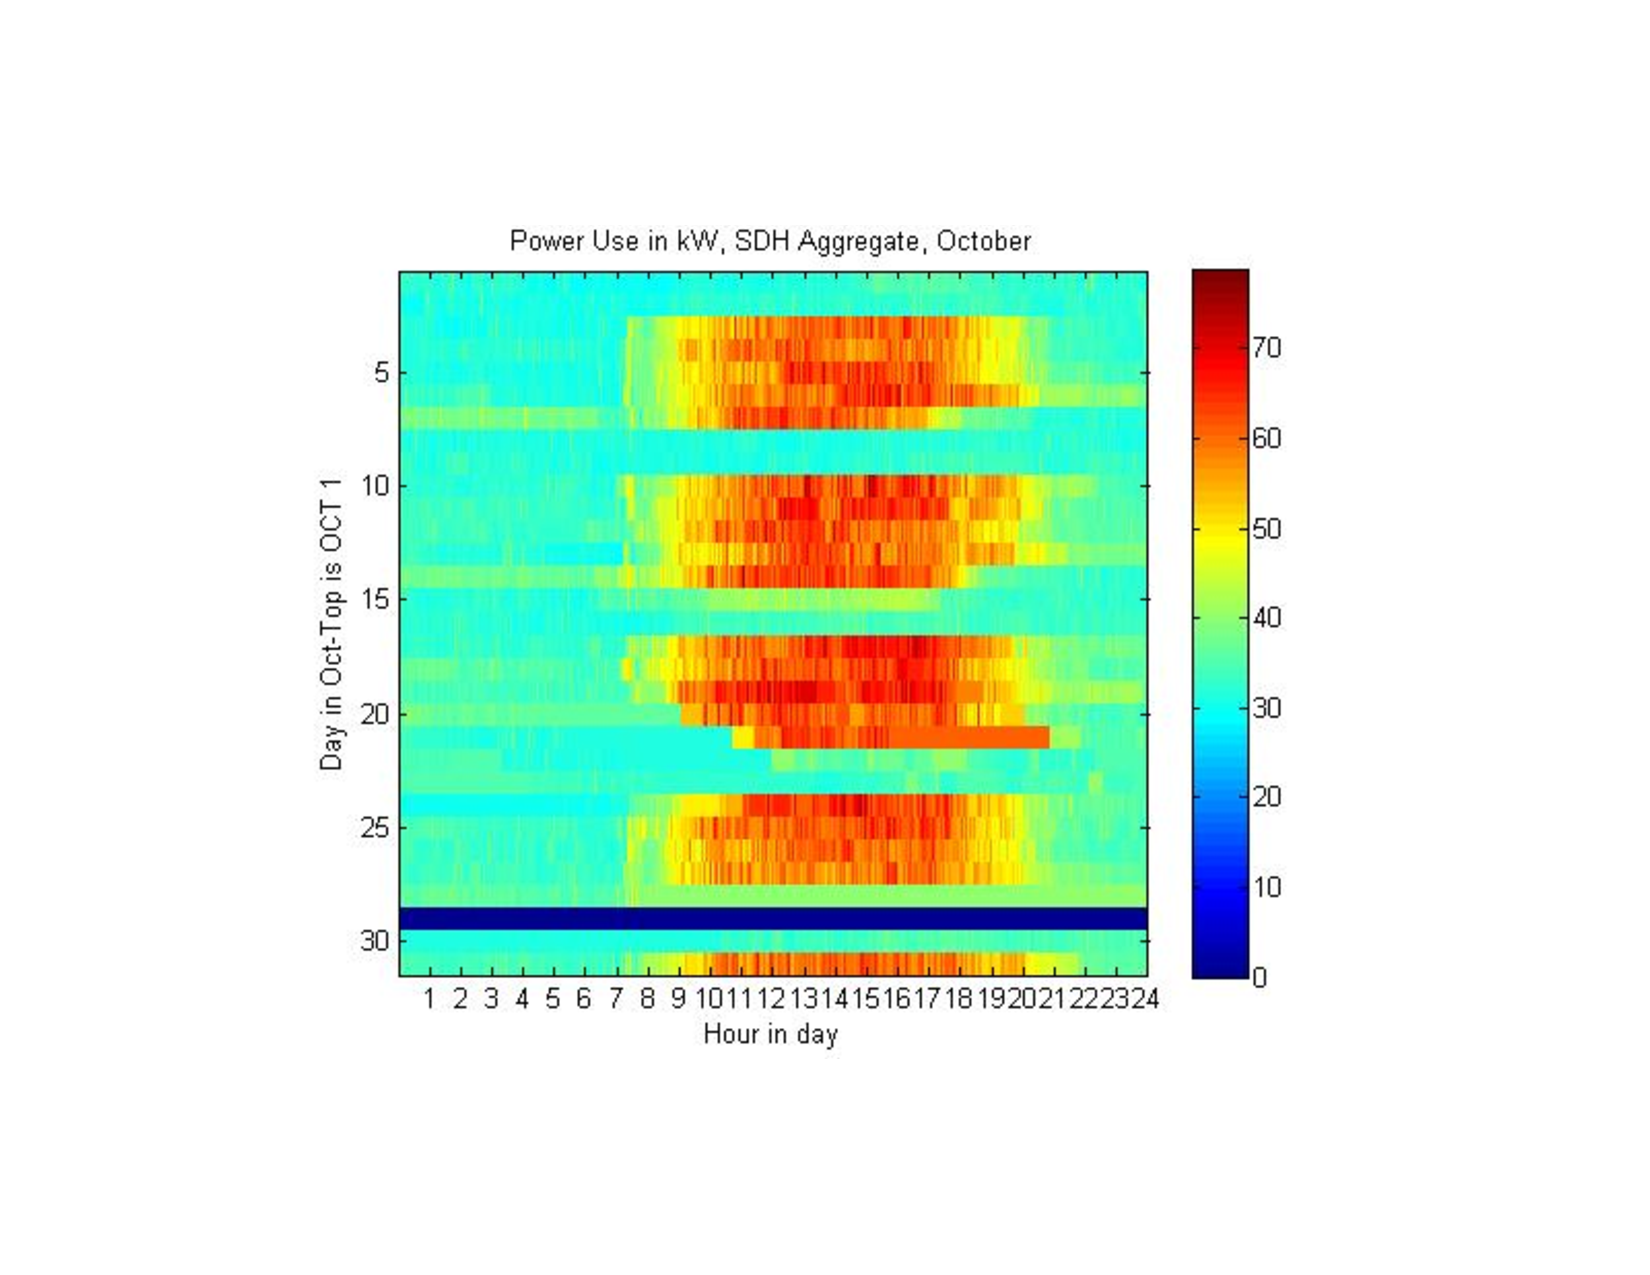
\includegraphics[scale=0.4]{figs/heatgrid}
% \caption{}
% \label{channelcomp}
% \end{center}
% \end{figure}

\begin{figure}[htb!]
\begin{center}
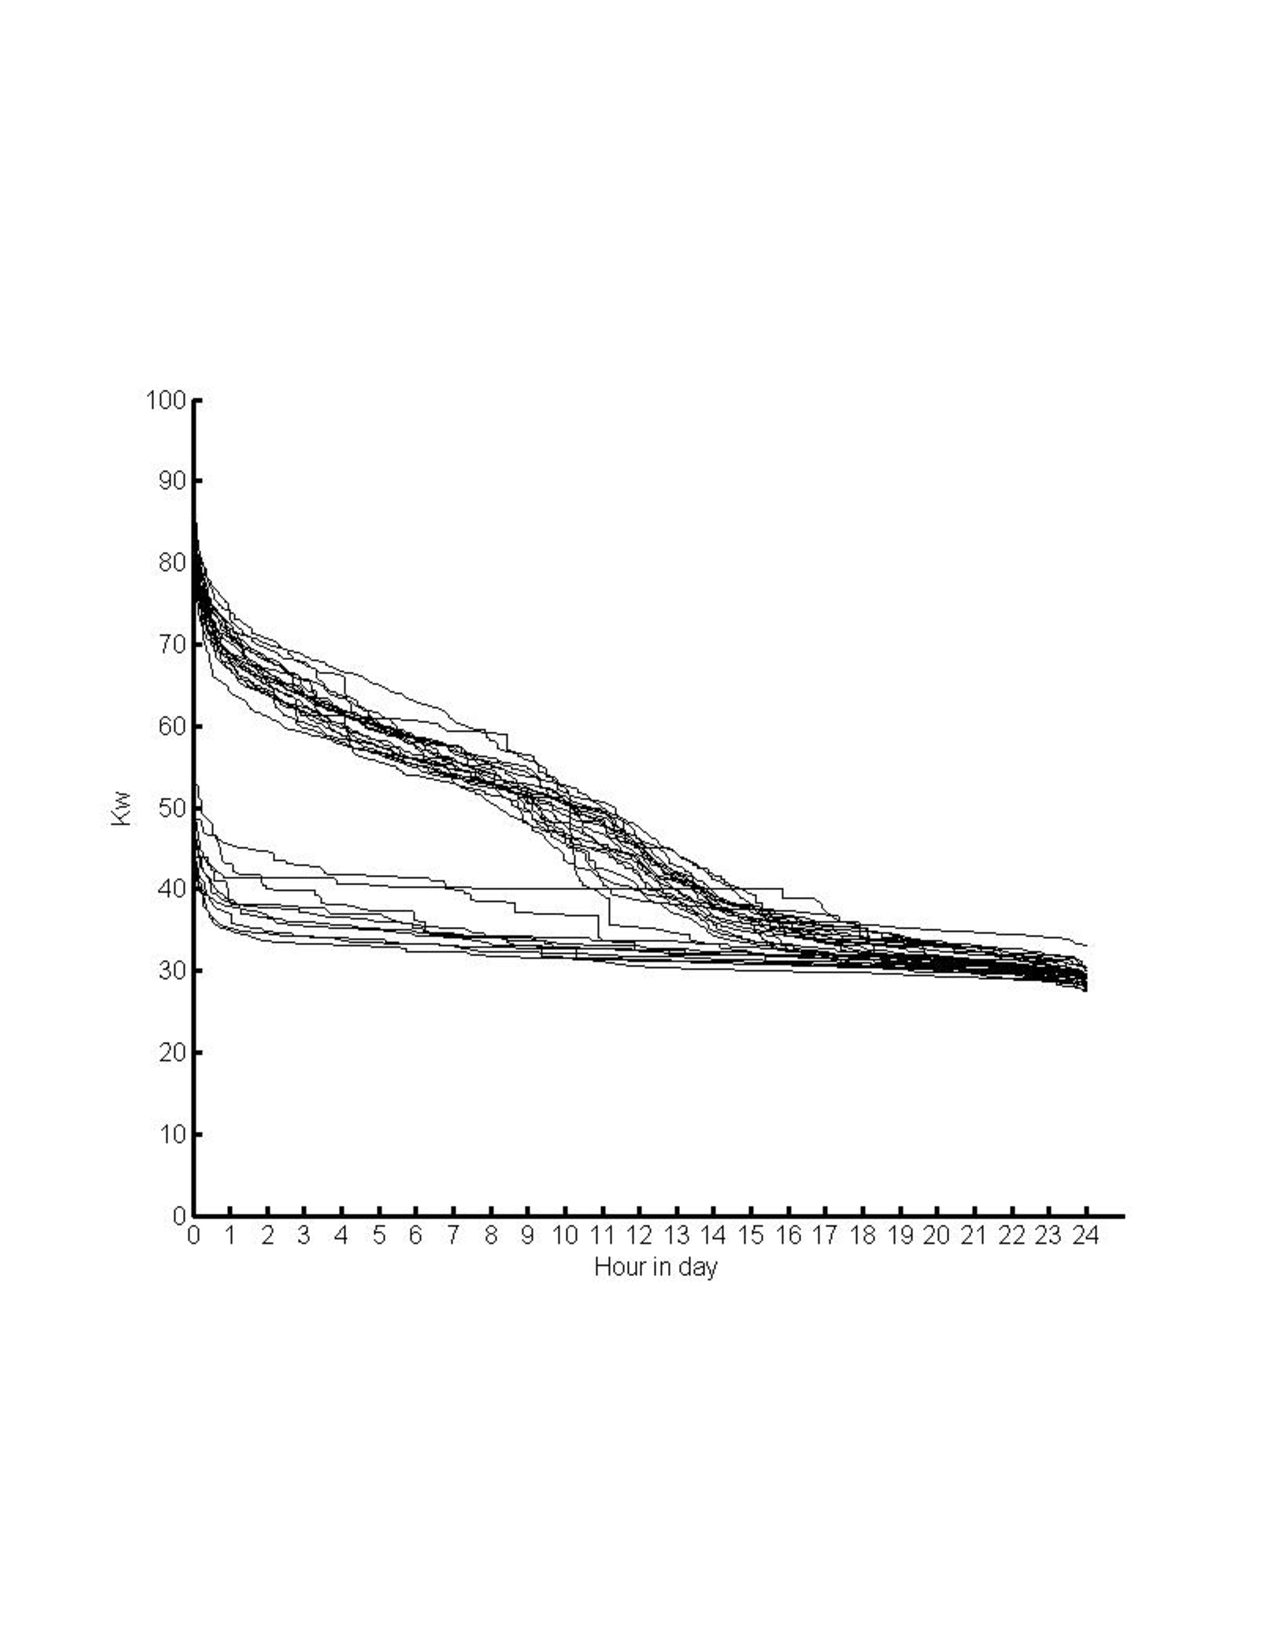
\includegraphics[scale=0.4]{figs/LoadDurationCurvesWholeBuildingBLACK}
\caption{Load duration curves.}
\label{fig:ldc}
\end{center}
\end{figure}

Figure~\ref{fig:ldc} shows the load duration curve for each day in the month of October.  The load duration
curve shows the number of hours in a 24-hour day that the load was at or above the level indicated on the 
y-axis.

\subsubsection{Issues}

Although many of the calculations are static and in large aggregates there were some fundamental challenges that
we encountered.  The first challenge is maintaining \emph{consistency} between the physical world and the virtual
representation of it.  About 16\% of the plug-load items we registered can be moved between locations by they owner
with relative frequency.  7\% (laptops) move quite often.  Maintaing of accurate view of what items are where
is a non-trivial with the right mechanisms in place.  Our approach in this case is to depend on the ubiquity of
smartphones and participants.  If a person moves an item from one location to another, they can swipe the item out
of the current location and swipe the item back in at the new location.  In addition, we take advantage of
natural usage patterns.  People tend to forget to swipe items out of their current location, so we leverage the
second swipe (swipe-in) to imply the first operation (swipe-out).  If the item was connected to a meter, we unbind the item
from the old meter before swiping the item out.  

We are currently working on adjusting the timestamp based on this action as well.
From the trace of the meter we can see when the item was unplugged (or turned off).  The sudden drop in power
reading could be used to mark the point of disconnection.  However, this only gets us part of the solution.  If the person
forgets multiple actions, it become more difficult to determine what has occurred.  For example, if a lamp is plugged
into a meter in room 1 and they unplug it from the meter, plug another device into it, and move the lamp to
another location, the unplug time is not clear.  If the new device draws power, we cannot tell the difference between
the trace generated from the new device versus the old device.  This is a non-intrusive load-trace classification
problem and beyond the scope of the current project.

% \begin{itemize}
% %\item Context tracking:  Localization through a swipe or implicit location change through natural action
% \item tracking mobile users
% \item tracking mobile objects
% 	\begin{itemize}
% 	\item devices
% 	\item meters
% 	\end{itemize}
% \end{itemize}